
\documentclass{article}

% Packages
\usepackage[utf8]{inputenc}
\usepackage[
    left=2.5cm,
    right=2.5cm,
    top=2.5cm,
    bottom=2.5cm
]{geometry}

\usepackage{graphicx}
\usepackage{subcaption}
\usepackage{listings}
\usepackage{makecell}
\usepackage{hyperref}
\usepackage[table]{xcolor}
\usepackage{placeins}
\usepackage{verbatim}
\usepackage{amsmath}
\usepackage{amssymb}
\usepackage{booktabs}
\usepackage{stmaryrd}
\usepackage[edges]{forest}
\usepackage{float}
\usepackage{tabularx}
\usepackage{longtable}
\usepackage{overpic}
\usepackage{fancyhdr}
\usepackage{setspace}

\definecolor{tableheader}{HTML}{EBF1F2}

\setlength{\parindent}{0pt}

% Define VS Code-like colors
\definecolor{vscodeBackground}{RGB}{30,30,30}
\definecolor{vscodeKeyword}{RGB}{197,134,192}
\definecolor{vscodeString}{RGB}{206,145,120}
\definecolor{vscodeComment}{RGB}{106,153,85}
\definecolor{vscodeNumber}{RGB}{181,206,168}
\definecolor{vscodeFunction}{RGB}{220,220,170}
\definecolor{vscodeTag}{RGB}{86,156,214}
\definecolor{vscodeAttribute}{RGB}{156,220,254}
\definecolor{vscodeText}{RGB}{212,212,212}
\definecolor{vscodeLineNumber}{RGB}{133,133,133}

% HTML style
\lstdefinestyle{htmlStyle}{
  language=HTML,
  backgroundcolor=\color{vscodeBackground},
  basicstyle=\ttfamily\small\color{vscodeText},
  keywordstyle=\color{vscodeTag}\bfseries,
  stringstyle=\color{vscodeString},
  commentstyle=\color{vscodeComment}\itshape,
  identifierstyle=\color{vscodeAttribute},
  numbers=left,
  numberstyle=\tiny\color{vscodeLineNumber},
  numbersep=10pt,
  stepnumber=1,
  showstringspaces=false,
  breaklines=true,
  frame=single,
  frameround=tttt,
  rulecolor=\color{vscodeLineNumber},
  tabsize=2,
  captionpos=b,
  breakatwhitespace=false,
  xleftmargin=2em,
  framexleftmargin=1.5em,
  moredelim=[s][\color{vscodeTag}]{<}{>},
  morestring=[b]",
  morestring=[b]',
  literate=
    {0}{{{\color{vscodeNumber}0}}}1
    {1}{{{\color{vscodeNumber}1}}}1
    {2}{{{\color{vscodeNumber}2}}}1
    {3}{{{\color{vscodeNumber}3}}}1
    {4}{{{\color{vscodeNumber}4}}}1
    {5}{{{\color{vscodeNumber}5}}}1
    {6}{{{\color{vscodeNumber}6}}}1
    {7}{{{\color{vscodeNumber}7}}}1
    {8}{{{\color{vscodeNumber}8}}}1
    {9}{{{\color{vscodeNumber}9}}}1
}

% Python style
\lstdefinestyle{pythonStyle}{
  language=Python,
  backgroundcolor=\color{vscodeBackground},
  basicstyle=\ttfamily\small\color{vscodeText},
  keywordstyle=\color{vscodeKeyword}\bfseries,
  stringstyle=\color{vscodeString},
  commentstyle=\color{vscodeComment}\itshape,
  identifierstyle=\color{vscodeText},
  numbers=left,
  numberstyle=\tiny\color{vscodeLineNumber},
  numbersep=10pt,
  stepnumber=1,
  showstringspaces=false,
  breaklines=true,
  frame=single,
  frameround=tttt,
  rulecolor=\color{vscodeLineNumber},
  tabsize=4,
  captionpos=b,
  breakatwhitespace=false,
  xleftmargin=2em,
  framexleftmargin=1.5em,
  morekeywords={as,with,self,True,False,None},
  emphstyle=\color{vscodeFunction},
  morestring=[b]",
  morestring=[b]',
  morestring=[b]""",
  literate=
    {0}{{{\color{vscodeNumber}0}}}1
    {1}{{{\color{vscodeNumber}1}}}1
    {2}{{{\color{vscodeNumber}2}}}1
    {3}{{{\color{vscodeNumber}3}}}1
    {4}{{{\color{vscodeNumber}4}}}1
    {5}{{{\color{vscodeNumber}5}}}1
    {6}{{{\color{vscodeNumber}6}}}1
    {7}{{{\color{vscodeNumber}7}}}1
    {8}{{{\color{vscodeNumber}8}}}1
    {9}{{{\color{vscodeNumber}9}}}1
}

% Header and footer
\pagestyle{fancy}
\fancyhf{}
\fancyfoot[L]{Imperial Business School - Analytics in Business, Summer 2026}
\fancyfoot[R]{\thepage}

\begin{document}

%TC:ignore
\begin{titlepage}
\pagestyle{empty}

\begin{center}

\vspace*{1.5cm}

{\Large Imperial College Business School}\\[0.3cm]

{\large Analytics in Business Consulting Project}\\[0.5cm]

\rule{\textwidth}{1.2pt}

\vspace{0.5cm}

{\Huge Dynamic Pricing Feasibility Assessment for CeramTec}\\[0.1cm]

\vspace{0.2cm}

\rule{\textwidth}{1.2pt}


\vspace{1cm}

{\large CID: 02023817, 06070918, 06066256, 06054938}\\[0.2cm]
{\large Date: 17th August 2026}\\[0.2cm]

\end{center}

\end{titlepage}
%TC:endignore



\pagestyle{fancy} 

\singlespacing

\setcounter{page}{1} % reset page counter to 1



\vspace{0.5em}

\section*{Executive Summary}


\section*{Acknowledgments}

\newpage
\tableofcontents
\newpage

\section{Introduction}

CeramTec is a global manufacturer of advanced technical ceramics and a leading supplier of ceramic components for orthopaedic implants. This report focuses on CeramTec's ceramic bearings used in total hip replacements and investigates whether a data-driven dynamic pricing strategy could improve the company's pricing decisions across different markets and customers.

A total hip implant is a prosthetic device that replaces a damaged hip joint to restore mobility and relieve pain. As illustrated in Figure~\ref{fig:hip_implant}, the implant consists of several components, including the femoral stem, femoral head, acetabular shell, and acetabular liner. The bearing is the articulating interface between the femoral head and the acetabular liner, enabling smooth movement of the joint.

\begin{figure}[H]
\centering
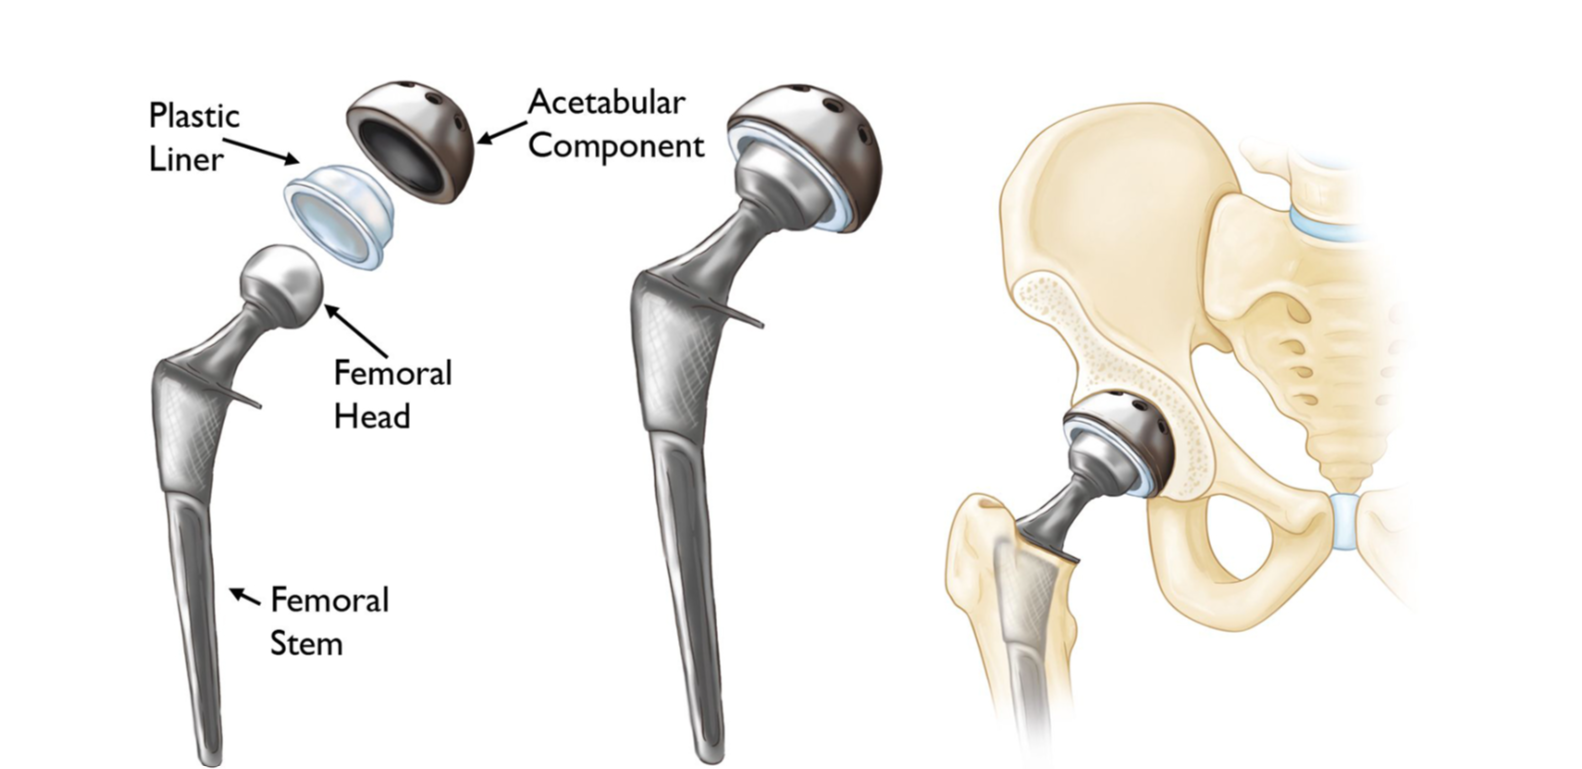
\includegraphics[width=0.8\linewidth]{introduction/hip_implant.png}
\caption{Components of a total hip implant.}
\label{fig:hip_implant}
\end{figure}

The choice of bearing material (such as ceramic-on-ceramic, ceramic-on-polyethylene, or metal-on-polyethylene) has a significant impact on wear performance, implant longevity, revision risk, and long-term patient outcomes. These characteristics also influence the economic value of the implant, making the bearing a key driver of both clinical outcomes and pricing decisions.

Although CeramTec currently prices its products primarily using a cost-based approach, it operates across markets with widely different reimbursement systems, procurement mechanisms, competitive environments, and customer profiles. These differences suggest that a uniform pricing strategy may not fully capture customers' willingness to pay or the value delivered by ceramic bearings. Furthermore, CeramTec serves multiple OEM customers with different market positions and product portfolios, creating additional opportunities for differentiated pricing.

The objective of this project is therefore to assess the feasibility of implementing a data-driven pricing strategy for CeramTec's ceramic hip bearings. To support this objective, we developed a comprehensive external-data foundation covering reimbursement systems, procurement, procedure volumes, clinical evidence, macroeconomic indicators, and OEM characteristics across four strategic markets. This evidence is subsequently combined with internal data to support market segmentation and predictive pricing models.


\section{Business Context and Project Scope}

\subsection{CeramTec in the value chain}

CeramTec operates as a \textbf{B2B component supplier} in the orthopaedic value chain: it manufactures high-performance ceramic femoral heads and acetabular liners that implant OEMs integrate into complete hip systems. Hospitals and purchasing organisations negotiate with OEMs under country-specific reimbursement and procurement rules; CeramTec's commercial challenge is therefore \textbf{two-level}---defending component value to OEM buyers whose own margins are capped by payer ceilings, tender outcomes, and episode-based reimbursement.

\subsubsection{Customer base and competitive landscape}

The project's key-account work focuses on five global OEMs for which external financial and innovation signals were assembled (SEC XBRL, patent snapshots, reimbursement exposure):

\begin{itemize}
  \item \textbf{Stryker Corporation} (USA) --- high-volume orthopaedics; robotics-led premium positioning
  \item \textbf{DePuy Synthes / J\&J MedTech} (USA) --- global leader; significant China VBP exposure
  \item \textbf{Zimmer Biomet Holdings} (USA) --- large incumbent; cost discipline under US hospital pressure
  \item \textbf{Smith+Nephew plc} (UK/US ADR) --- medium-high ceramic relevance; Europe reimbursement-aware
  \item \textbf{Medacta International} (Switzerland) --- smaller scale; innovation-partner profile in Europe
\end{itemize}

\textcolor{red}{[TODO: complete the full CeramTec OEM customer list and account revenue shares from internal CRM/sales data.]}

Substitute ceramic and technical-ceramics suppliers identified in the external register include CoorsTek, HiPer Medical, Kyocera Medical, Enovis/Mathys (OEM with own ceramic line), and several China-based suppliers (Suntech/Cericare, Three-Circle, Arthrone, TrendTec, Yukun) plus G.\ Surgiwear (India). \textcolor{red}{[TODO: validate competitive overlap and market-share estimates with CeramTec commercial intelligence.]}

Table~\ref{tab:positioning} summarises how CeramTec positions relative to selected OEM customers and ceramic competitors. CeramTec's differentiation is as a \textbf{dedicated ceramic-component specialist} with the BIOLOX$^{\textregistered}$ product family, rather than as a full-system implant OEM or a general technical-ceramics conglomerate.

\begin{table}[H]
\centering
\small
\caption{Positioning snapshot: CeramTec vs selected OEM customers and ceramic competitors}
\label{tab:positioning}
\begin{tabular}{@{}p{2.2cm}p{1.6cm}p{4.2cm}p{4.8cm}@{}}
\toprule
\textbf{Firm} & \textbf{Type} & \textbf{Market role} & \textbf{vs.\ CeramTec} \\
\midrule
CeramTec & Supplier & BIOLOX ceramic heads/liners for hip OEMs & Reference player; alumina/ZTA ceramic IP and scale \\
Stryker & OEM customer & Full hip systems; premium robotics portfolio & Major volume account; MS-DRG cost pressure \\
DePuy Synthes & OEM customer & Global orthopaedics; China manufacturing & Strategic partner; VBP ceiling risk \\
Zimmer Biomet & OEM customer & Value + premium hip lines & Defend account; dual-sourcing risk \\
Smith+Nephew & OEM customer & Sports med.\ + orthopaedics & Nurture; smaller ceramic volume \\
Medacta & OEM customer & Surgeon-centric EU OEM & Grow; innovation proximity \\
CoorsTek & Competitor & Broad technical ceramics incl.\ medical & Generalist; US-centric \\
Kyocera Medical & Competitor & Orthopaedic + dental ceramics & Vertically integrated Japanese player \\
HiPer Medical & Competitor & Swiss ceramic hip components & European boutique competitor \\
Enovis/Mathys & Competitor/OEM & Own ceramic femoral heads & OEM-owned ceramic supply \\
\bottomrule
\end{tabular}
\end{table}

Data-driven pricing is essential in this context because OEM willingness-to-pay varies with their financial health, innovation intensity, geographic reimbursement exposure, and competitive sourcing options---none of which can be inferred from CeramTec's internal cost base alone.

\subsection{Hip bearing products}

CeramTec's hip portfolio centres on the \textbf{BIOLOX$^{\textregistered}$} family of bioceramic components supplied to OEMs, who then offer them in different \textbf{bearing couples}:

\begin{itemize}
  \item \textbf{BIOLOX$^{\textregistered}$ forte} --- alumina ceramic; established option for femoral heads in ceramic-on-polyethylene (CoP) systems
  \item \textbf{BIOLOX$^{\textregistered}$ delta} --- zirconia-toughened alumina (ZTA) matrix composite; used in premium CoP and ceramic-on-ceramic (CoC) constructs with improved fracture toughness
\end{itemize}

\textcolor{red}{[TODO: confirm current product SKU list, sizes, and any additional BIOLOX variants from CeramTec product catalogue.]}

Clinically, the bearing couple determines wear debris, fracture risk, and long-term survivorship. CoC couplings minimise polyethylene wear but require precise engineering and patient selection; CoP remains the volume segment in most markets. Registry data collected in Phase~1 (US AJRR, Italy RIAP, France Open LPP, China VBP proxies) show materially different ceramic-involved shares across markets---directly relevant to CeramTec's addressable premium volume.

Revision risk, wear behaviour, and long-term outcomes are therefore not only clinical endpoints but \textbf{pricing levers}: where registries and literature associate higher ceramic adoption with lower revision burden (H1 in our hypothesis table: Pearson $r \approx -0.99$ across four country means, $n=4$), CeramTec can support OEM value stories for premium components. \textcolor{red}{[TODO: add CeramTec-approved clinical evidence claims and any proprietary survivorship data.]}

\begin{figure}[H]
\centering
\fbox{\parbox[c][3.5cm][c]{0.42\textwidth}{\centering\textcolor{gray}{[Image placeholder:\\BIOLOX femoral head]}}}
\hfill
\fbox{\parbox[c][3.5cm][c]{0.42\textwidth}{\centering\textcolor{gray}{[Image placeholder:\\BIOLOX acetabular liner / insert]}}}
\caption{CeramTec BIOLOX hip components (images to be added).}
\label{fig:biolox-placeholders}
\end{figure}

\begin{figure}[H]
\centering
\fbox{\parbox[c][3cm][c]{0.9\textwidth}{\centering\textcolor{gray}{[Image placeholder: bearing-couple schematic --- CoP vs CoC vs MoP]}}}
\caption{Bearing-surface couples using ceramic components (schematic to be added).}
\label{fig:bearing-couples-placeholder}
\end{figure}

\subsubsection{Current pricing approach}

CeramTec currently prices its bearings on a cost-plus basis: production cost plus a margin.

\begin{itemize}
    \item \textcolor{red}{[TODO: obtain average/typical margin applied, and whether it varies by product line or account]}
    \item \textcolor{red}{[TODO: confirm whether any market- or OEM-level differentiation already exists informally]}
\end{itemize}

Given that willingness-to-pay and margin headroom differ materially by country, payer system, and OEM segment, a single global cost-plus price cannot capture differences such as reimbursement ceilings in France, regional tariff heterogeneity in Italy, or VBP-linked constraints in China. Each OEM also has a distinct market positioning and product range, motivating differentiation by buyer as well as by market.

\subsection{Project Objectives}

The project objective is to design a \textbf{data-driven pricing strategy} for CeramTec's hip implant bearing components: moving from intuition-led OEM negotiations to evidence-backed segmentation by market, payer environment, and account profile.

\subsection{Scope}

\textbf{Geographic markets and accounts:} the analysis covers 4 countries (USA, China, France, Italy) and, per CeramTec direction, 16 OEM accounts.

\begin{itemize}
    \item \textcolor{red}{[TODO: reconcile "16 OEMs" scope with the 5 key accounts currently profiled in \S2.1.1 -- clarify whether the remaining 11 are lower priority, unprofiled, or out of Phase~1's data scope]}
\end{itemize}

Given $16 \times 4 = 64$ potential market--OEM price points, a data-driven, segmentation-based approach is preferred over ad hoc account-by-account negotiation.

\textbf{OEM accounts:} the five key accounts profiled above, with financial and patent signals from SEC EDGAR (where available) and structured Steckbrief templates in \texttt{data/external/oem/account\_profiles/}.

\textbf{Evidence categories:} thirteen families in the External Data Register---FX, materials/energy, reimbursement, procurement, waiting times, surgery volumes, bearing mix, clinical/revision evidence, macro health spending, medtech benchmarks, OEM fundamentals, and competitors---totalling 51 tracked source rows.

\textbf{Pricing dimensions analysed:} input-cost pass-through (materials, energy, FX), payer budget ceilings (episode and device tariffs), observed procurement competition, demand volume and bearing-mix evolution, revision-related value, OEM financial capacity, and competitive ceramic supply.

A core deliverable beyond static analysis is a \textbf{maintainable external-data capability}: reproducible scraping/processing scripts, a synchronized team register (Google Sheet $\rightarrow$ repo), one EDA notebook per data category, and cross-category learnings notebooks for combined analysis.

\subsection{Project phases}

\begin{table}[H]
\centering
\small
\caption{Project phases and main deliverables}
\label{tab:phases}
\begin{tabular}{@{}p{1.4cm}p{4.8cm}p{6.8cm}@{}}
\toprule
\textbf{Phase} & \textbf{Objective} & \textbf{Key deliverables (status)} \\
\midrule
1 & Build external evidence foundation and first market signals & External Data Register; 13-category data pipeline; market panel (US/FR/IT/CN); 7 hypotheses; 5 Key Account Steckbriefe; Phase~1 charts (\texttt{outputs/phase1/}); category EDA notebooks --- \textbf{done} \\
2 & Enrich data quality and join internal CeramTec pricing & Registry upgrades (US HCUP/AJRR, CN CJAR, FR ATIH); internal OEM price series; supervised pricing model; CRM completion of account profiles --- \textcolor{red}{[in progress / TODO]} \\
3 & Test pricing hypotheses and build segmentation framework & Formal tests of H1--H7 (OLS, Chow breaks, K-means OEM clusters); market--OEM pricing segmentation rules --- \textcolor{red}{[TODO: confirm Phase 3 scope with CeramTec]} \\
4 & Operationalise pricing recommendations & \textcolor{red}{[TODO: define Phase 4 deliverables --- e.g.\ negotiation playbooks, pricing tool/dashboard, rollout plan]} \\
\bottomrule
\end{tabular}
\end{table}

Phase~1 established the structured, reproducible backbone required for later phases: without a maintained register and automated retrieval, any segmentation model would age quickly as reimbursement rules, VBP rounds, and registry publications change. Subsequent phases depend on \textcolor{red}{[TODO: CeramTec internal bearing price history and account-level contract data]} to move from external proxies to actionable list-price and discount recommendations.


\section{Phase 1}

Phase 1 starts from a clear initial situation: CeramTec had no centralized external-data system for pricing intelligence. Relevant signals existed across public institutions, registries, procurement portals, reimbursement schedules, macro databases, and company disclosures, but they were fragmented, inconsistent in format, and difficult to use in negotiation timelines.

Our solution was to build an end-to-end external evidence pipeline across all key pricing dimensions. Instead of collecting one-off files, we organized sources into a unified register and implemented reproducible retrieval and processing scripts so the dataset can be refreshed, extended, and maintained over time. This turns Phase 1 from a static deliverable into a durable capability that can keep tracking market evolution after the project period.

\subsection{Categorisation of the data}

The external evidence base is structured into 13 categories covering the full pricing logic: FX, material and energy cost pressure, reimbursement ceilings, public procurement prices, waiting times, surgery volumes, bearing mix, revision and clinical evidence, macro health spending, medtech benchmarks, OEM fundamentals, and competitor context. This structure ensures each pricing hypothesis can be linked to a specific and traceable evidence family rather than ad hoc assumptions.

At the register level, the current synchronized version tracks 51 rows of sources and datasets across these categories. Beyond the raw count, the workload was substantial because each source required separate handling rules (API pulls, structured CSV retrieval, PDF extraction, registry harmonization, or proxy construction where official data was incomplete). The result is a broad multi-market evidence map rather than a narrow single-dataset analysis.

Data acquisition was particularly difficult in healthcare due to uneven transparency and highly heterogeneous publication formats. Open machine-readable datasets are limited for several critical topics, many key values are embedded in long institutional PDFs, and time coverage can be irregular by country and year. In practice, this required country-specific retrieval strategies, explicit quality flags, and carefully documented partial/proxy coverage where full registry data was not available.

\subsection{Exploratpry data analysis}

The exploratory analysis phase translated the retrieved evidence into first-order market signals. Initial plots focused on identifying drivers that plausibly explain pricing pressure and negotiation context: procedure volume trajectories, bearing-mix evolution, reimbursement ceilings versus observed procurement dynamics, and input-cost indicators (materials, energy, FX). This first signal layer is not intended as a final causal model; it establishes which variables are most promising for deeper pricing segmentation in later phases.


\subsection{Maintainability and durability of the solution}

Maintainability was a design requirement from the start. We implemented reusable scraping and processing scripts so data refreshes can be run as a standard workflow rather than rebuilt manually each cycle. Concretely, the project now supports one-command orchestration for retrieval and processing, plus a synchronized external register that documents source status, market scope, and update frequency. This makes it feasible to ingest new releases regularly, preserve methodological consistency, and keep pricing evidence current over time.

\section{Phase 2}

inspect internal data and relevant feature engineering

\section{Phase 3}

market + customer segmentation using clustering approach

\section{Phase 4}

predictive model

\section{Conclusion}

\appendix
% <<REGISTER_BEGIN>>
\section{External Data Source Register}
\label{app:external-data-register}

This appendix mirrors the team Google Sheet \textit{External Data Register} (Drive folder \texttt{data/external}). Last synced: 2026-07-06.

\subsection{Status legend}
\begin{tabular}{@{}ll@{}}
\toprule
\textbf{Status} & \textbf{Meaning} \\
\midrule
\textcolor{green!60!black}{Retrieved} & Automated fetch works; data on disk or in processed outputs \\
\textcolor{orange!85!black}{Partial} & Some data or proxies only; not a full registry extract \\
\textcolor{gray}{Todo} & Not yet retrieved \\
\bottomrule
\end{tabular}

\subsection{Currency exchange rates}
Cross-border pricing risk — how EUR-based production cost translates into OEM selling prices and payer ceilings in USD, GBP, CNY, etc.\\[0.5em]

\small
\setlength{\tabcolsep}{4pt}
\renewcommand{\arraystretch}{1.15}
\begin{longtable}{@{}p{2.1cm}p{2.4cm}p{1.4cm}p{1.5cm}p{1.3cm}p{5.2cm}@{}}
\toprule
\textbf{Folder} & \textbf{Dataset} & \textbf{Status} & \textbf{Market} & \textbf{Freq.} & \textbf{Comments} \\
\midrule
\endhead
\midrule
\multicolumn{6}{r}{\textit{Continued on next page}} \\
\endfoot
\bottomrule
\endlastfoot
fx/ & ECB FX & \textcolor{green!60!black}{Retrieved} & Global & Daily & EUR vs USD, GBP, CNY, JPY, CHF \\
\end{longtable}
\normalsize

\subsection{Material \& Commodity prices}
Input-cost pressure on ceramic/metal components\\[0.5em]

\small
\setlength{\tabcolsep}{4pt}
\renewcommand{\arraystretch}{1.15}
\begin{longtable}{@{}p{2.1cm}p{2.4cm}p{1.4cm}p{1.5cm}p{1.3cm}p{5.2cm}@{}}
\toprule
\textbf{Folder} & \textbf{Dataset} & \textbf{Status} & \textbf{Market} & \textbf{Freq.} & \textbf{Comments} \\
\midrule
\endhead
\midrule
\multicolumn{6}{r}{\textit{Continued on next page}} \\
\endfoot
\bottomrule
\endlastfoot
materials/ & Fred metals/PPI & \textcolor{green!60!black}{Retrieved} & Global & Monthly & Surgical-appliance PPI, alumina/aluminum/titanium/nickel shapes, IMF metal prices \\
 & World Bank CMO & \textcolor{green!60!black}{Retrieved} & Global & Monthly & Energy and commodity indices; monthly material prices \\
 & USGS MCS (Mineral Commodity Summaries) & \textcolor{green!60!black}{Retrieved} & Global & Annual & Annual unit values: Al, Cr, Co, Fe, Pb, Mo, Ni, Sn, Ti, Zn, Zr/Hf \\
\end{longtable}
\normalsize

\subsection{Energy \& Manufacturing PPI}
Firing/sintering and supply-chain inflation compressing OEM implant margins\\[0.5em]

\small
\setlength{\tabcolsep}{4pt}
\renewcommand{\arraystretch}{1.15}
\begin{longtable}{@{}p{2.1cm}p{2.4cm}p{1.4cm}p{1.5cm}p{1.3cm}p{5.2cm}@{}}
\toprule
\textbf{Folder} & \textbf{Dataset} & \textbf{Status} & \textbf{Market} & \textbf{Freq.} & \textbf{Comments} \\
\midrule
\endhead
\midrule
\multicolumn{6}{r}{\textit{Continued on next page}} \\
\endfoot
\bottomrule
\endlastfoot
materials/ & FRED energy & \textcolor{green!60!black}{Retrieved} & Global & Monthly/Daily & Natural gas, industrial electricity (ceramics processing cost pressure) \\
 & FRED surgical-appliance / orthopedic PPI & \textcolor{green!60!black}{Retrieved} & Global & Monthly & Manufacturing inflation pressure on OEM implant margins \\
\end{longtable}
\normalsize

\subsection{Reimbursement rates \& amounts}
Money-In: Total insurer/payer revenue paid to the hospital for the entire episode of care. Sets the absolute budgetary ceiling for the procedure and device.\\[0.5em]

\small
\setlength{\tabcolsep}{4pt}
\renewcommand{\arraystretch}{1.15}
\begin{longtable}{@{}p{2.1cm}p{2.4cm}p{1.4cm}p{1.5cm}p{1.3cm}p{5.2cm}@{}}
\toprule
\textbf{Folder} & \textbf{Dataset} & \textbf{Status} & \textbf{Market} & \textbf{Freq.} & \textbf{Comments} \\
\midrule
\endhead
\midrule
\multicolumn{6}{r}{\textit{Continued on next page}} \\
\endfoot
\bottomrule
\endlastfoot
reimbursement/ & CMS MS-DRG & \textcolor{green!60!black}{Retrieved} & US & Annual & Medicare (public funds) episode payment for hip/knee arthroplasty (DRG 470 family) \\
 & FAIR Health / Definitive & \textcolor{gray}{Todo} & US & Continuous & Private/commercial insurance claims database for private reimbursement benchmarks \\
 & ATIH GHS (the stay at the hospital) & \textcolor{green!60!black}{Retrieved} & France & Annual & Public-hospital episode tariffs (GHM 08C hip family) \\
 & LPPR (Liste des Produits) (the device) & \textcolor{green!60!black}{Retrieved} & France & Continuous & Specific national maximum reimbursement limits for medical devices/implants \\
 & Regional DRG (The Stay + Device) & \textcolor{orange!85!black}{Partial} & Italy & Annual & Inpatient DRG (e.g. Piedmont 209) + national prosthetic list, note that system in italy is highly regionalized \\
 & Nomenclatore / Regional Reference Lists (The Device Cap) & \textcolor{gray}{Todo} & Italy & Dynamic & the Italian health system is highly regionalized, the regions (like Lombardy or Veneto) publish specific medical device tariff lists (often referred to as Tetti di spesa or reference prices) \\
 & NHSA VBP ceiling & \textcolor{orange!85!black}{Partial} & China & per-round & Public-hospital implant max bids (CoC/CoP/MoP differentiated) \\
\end{longtable}
\normalsize

\subsection{Public procurement awards}
Money-Out: Actual transaction price paid by hospitals/tenders to the implant manufacturer for the hardware. Reflects real market competition and discounts.\\[0.5em]

\small
\setlength{\tabcolsep}{4pt}
\renewcommand{\arraystretch}{1.15}
\begin{longtable}{@{}p{2.1cm}p{2.4cm}p{1.4cm}p{1.5cm}p{1.3cm}p{5.2cm}@{}}
\toprule
\textbf{Folder} & \textbf{Dataset} & \textbf{Status} & \textbf{Market} & \textbf{Freq.} & \textbf{Comments} \\
\midrule
\endhead
\midrule
\multicolumn{6}{r}{\textit{Continued on next page}} \\
\endfoot
\bottomrule
\endlastfoot
procurement/ & TED (EU) & \textcolor{green!60!black}{Retrieved} & EU & Continuous & EU-orthopaedic procurement notices \\
 & BOAMP / UniHA / Resah & \textcolor{gray}{Todo} & France & Continuous & French national public market announcements and hospital group purchasing awards \\
 & ANAC / Consip / Regional buyers & \textcolor{gray}{Todo} & Italy & Continuous & Italian contract database and regional central purchasing (ARIA, SoReSa) tender awards \\
 & Contracts Finder (UK) & \textcolor{green!60!black}{Retrieved} & UK & Continuous & UK public procurement awards \\
 & SAM.gov (VA Contracts) & \textcolor{gray}{Todo} & US & Continuous & Federal procurement awards for VA and military hospital implant contracts \\
 & ECRI / Definitive Healthcare & \textcolor{gray}{Todo} & US & Continuous & Aggregated hospital GPO transaction prices and private purchasing data \\
 & National Joint Procurement Office & \textcolor{gray}{Todo} & China & per-round & Official VBP winning bid results and volume allocations (Tianjin platform) \\
 & Yaozh / Pharmcube & \textcolor{gray}{Todo} & China & Continuous & Commercial aggregators scraping provincial VBP tender values and price cuts \\
\end{longtable}
\normalsize

\subsection{Waiting times}
Demand tension - elective backlog and capacity stress (UK orthopaedic proxy)\\[0.5em]

\small
\setlength{\tabcolsep}{4pt}
\renewcommand{\arraystretch}{1.15}
\begin{longtable}{@{}p{2.1cm}p{2.4cm}p{1.4cm}p{1.5cm}p{1.3cm}p{5.2cm}@{}}
\toprule
\textbf{Folder} & \textbf{Dataset} & \textbf{Status} & \textbf{Market} & \textbf{Freq.} & \textbf{Comments} \\
\midrule
\endhead
\midrule
\multicolumn{6}{r}{\textit{Continued on next page}} \\
\endfoot
\bottomrule
\endlastfoot
waiting\_times/ & NHS RTT & \textcolor{green!60!black}{Retrieved} & UK & Monthly & Elective surgery waiting times including trauma \& orthopaedic \\
\end{longtable}
\normalsize

\subsection{Number of sugeries}
Market size - THA (total hip arthroplasty) volume and rate per 100k population\\[0.5em]

\small
\setlength{\tabcolsep}{4pt}
\renewcommand{\arraystretch}{1.15}
\begin{longtable}{@{}p{2.1cm}p{2.4cm}p{1.4cm}p{1.5cm}p{1.3cm}p{5.2cm}@{}}
\toprule
\textbf{Folder} & \textbf{Dataset} & \textbf{Status} & \textbf{Market} & \textbf{Freq.} & \textbf{Comments} \\
\midrule
\endhead
\midrule
\multicolumn{6}{r}{\textit{Continued on next page}} \\
\endfoot
\bottomrule
\endlastfoot
surgeries/ & OECD Health — surgical procedures & \textcolor{green!60!black}{Retrieved} & Global & Annual & Cross-country procedure rates per 100k (hip replacement where available) \\
 & Eurostat — hospital discharges & \textcolor{green!60!black}{Retrieved} & EU & Annual & EU in-patient surgical operations; complements OECD for Europe \\
surgeries/reference/ & France reference overlays & \textcolor{orange!85!black}{Partial} & France & Ad hoc & Reference overlays where needed for panel consistency \\
 & Italy reference overlays & \textcolor{orange!85!black}{Partial} & Italy & Ad hoc & Reference overlays where needed for panel consistency \\
 & US reference & \textcolor{orange!85!black}{Partial} & US & Ad hoc & Fills OECD/registry gaps for Phase 1 panel \\
 & China reference & \textcolor{orange!85!black}{Partial} & China & Ad hoc & Fills OECD/registry gaps for Phase 1 panel \\
\end{longtable}
\normalsize

\subsection{Bearing mix}
Bearing mix (ceramic vs non-ceramic), revision burden, implant usage trend\\[0.5em]

\small
\setlength{\tabcolsep}{4pt}
\renewcommand{\arraystretch}{1.15}
\begin{longtable}{@{}p{2.1cm}p{2.4cm}p{1.4cm}p{1.5cm}p{1.3cm}p{5.2cm}@{}}
\toprule
\textbf{Folder} & \textbf{Dataset} & \textbf{Status} & \textbf{Market} & \textbf{Freq.} & \textbf{Comments} \\
\midrule
\endhead
\midrule
\multicolumn{6}{r}{\textit{Continued on next page}} \\
\endfoot
\bottomrule
\endlastfoot
surgeries/ajr & AJRR & \textcolor{green!60!black}{Retrieved} & US & Annual & Data for 2012 - 2024 \\
surgeries/riap & RIAP (Italy national) & \textcolor{green!60!black}{Retrieved} & Italy & Annual & 2015 - 2022 \\
reimbursement/lpp & open lpp (data.gouv.fr) & \textcolor{green!60!black}{Retrieved} & France & Annual & national reimbursement proxy contianing component-level, 2014 - 2024 \\
surgeries/cjar & CJAR / China proxies & \textcolor{green!60!black}{Retrieved} & China & Annual & 2021, 2022, 2024 (VBP demand + COA survey) \\
reimbursement/reference & NHSA VBP CoC/CoP tariffs & \textcolor{green!60!black}{Retrieved} & China & Per-round & Price ceiling by type, not volume share \\
\end{longtable}
\normalsize

\subsection{Revision \& clinical evidence}
Clinical value of longer-lasting bearings; revision-risk narrative\\[0.5em]

\small
\setlength{\tabcolsep}{4pt}
\renewcommand{\arraystretch}{1.15}
\begin{longtable}{@{}p{2.1cm}p{2.4cm}p{1.4cm}p{1.5cm}p{1.3cm}p{5.2cm}@{}}
\toprule
\textbf{Folder} & \textbf{Dataset} & \textbf{Status} & \textbf{Market} & \textbf{Freq.} & \textbf{Comments} \\
\midrule
\endhead
\midrule
\multicolumn{6}{r}{\textit{Continued on next page}} \\
\endfoot
\bottomrule
\endlastfoot
clinical\_evidence/pubmed & PubMed evidence exports & \textcolor{green!60!black}{Retrieved} & Global & Continuous & Survivorship, bearing-surface, China demographic citations \\
surgeries/reference/ & Revision-rate reference panel & \textcolor{orange!85!black}{Partial} & US / China / France / Italy & Ad hoc & Literature-anchored country-year revision proxies \\
\end{longtable}
\normalsize

\subsection{Macro health spending}
Payer budget envelope, public/private splot, OOP pressure\\[0.5em]

\small
\setlength{\tabcolsep}{4pt}
\renewcommand{\arraystretch}{1.15}
\begin{longtable}{@{}p{2.1cm}p{2.4cm}p{1.4cm}p{1.5cm}p{1.3cm}p{5.2cm}@{}}
\toprule
\textbf{Folder} & \textbf{Dataset} & \textbf{Status} & \textbf{Market} & \textbf{Freq.} & \textbf{Comments} \\
\midrule
\endhead
\midrule
\multicolumn{6}{r}{\textit{Continued on next page}} \\
\endfoot
\bottomrule
\endlastfoot
health\_spending/ & WHO GHED & \textcolor{green!60!black}{Retrieved} & Global & Annual & Total health spend, public/private split, out-of-pocket ratios by country \\
\end{longtable}
\normalsize

\subsection{MedTech sector benchmarks}
Orthopaedic market size context (public reports)\\[0.5em]

\small
\setlength{\tabcolsep}{4pt}
\renewcommand{\arraystretch}{1.15}
\begin{longtable}{@{}p{2.1cm}p{2.4cm}p{1.4cm}p{1.5cm}p{1.3cm}p{5.2cm}@{}}
\toprule
\textbf{Folder} & \textbf{Dataset} & \textbf{Status} & \textbf{Market} & \textbf{Freq.} & \textbf{Comments} \\
\midrule
\endhead
\midrule
\multicolumn{6}{r}{\textit{Continued on next page}} \\
\endfoot
\bottomrule
\endlastfoot
medtech\_benchmarks/ & MedTech Europe PDFs & \textcolor{orange!85!black}{Partial} & EU (mainly) & Annual & Public orthopaedic market facts \& figures (member-only detail not available) \\
 & US benchmark extracts (if available) & \textcolor{gray}{Todo} & US & Annual &  \\
 & China benchmark extracts (if available) & \textcolor{gray}{Todo} & China & Annual &  \\
\end{longtable}
\normalsize

\subsection{OEMs}
Clients, financial health, R\&D, innovation, account prirority\\[0.5em]

\small
\setlength{\tabcolsep}{4pt}
\renewcommand{\arraystretch}{1.15}
\begin{longtable}{@{}p{2.1cm}p{2.4cm}p{1.4cm}p{1.5cm}p{1.3cm}p{5.2cm}@{}}
\toprule
\textbf{Folder} & \textbf{Dataset} & \textbf{Status} & \textbf{Market} & \textbf{Freq.} & \textbf{Comments} \\
\midrule
\endhead
\midrule
\multicolumn{6}{r}{\textit{Continued on next page}} \\
\endfoot
\bottomrule
\endlastfoot
oem/ & SEC EDGAR & \textcolor{orange!85!black}{Partial} & Global & Quarterly/Annual & Revenue and R\&D for Stryker, Zimmer Biomet, J\&J/DePuy, Smith+Nephew, not all the OEMs, some of them are still missing, see the exhaustive list \\
oem/account\_profiles/ & account profiles & \textcolor{orange!85!black}{Partial} & Global & Ad hoc & Key account strategy files \\
oem/patents & Patent counts & \textcolor{orange!85!black}{Partial} & Global & Ad hoc & Innovation proxy snapshots \\
\end{longtable}
\normalsize

\subsection{Competitors}
Competitive set, subsitute bearing/ceramic suppliers\\[0.5em]

\small
\setlength{\tabcolsep}{4pt}
\renewcommand{\arraystretch}{1.15}
\begin{longtable}{@{}p{2.1cm}p{2.4cm}p{1.4cm}p{1.5cm}p{1.3cm}p{5.2cm}@{}}
\toprule
\textbf{Folder} & \textbf{Dataset} & \textbf{Status} & \textbf{Market} & \textbf{Freq.} & \textbf{Comments} \\
\midrule
\endhead
\midrule
\multicolumn{6}{r}{\textit{Continued on next page}} \\
\endfoot
\bottomrule
\endlastfoot
competitors & Competitor list / competitor datasets & \textcolor{gray}{Todo} & Global & Ad hoc & Nothing done, CeramTec should have internal data about their competitors, wait for their internal data to see what external data about the competitors need to be retrieved \\
\end{longtable}
\normalsize

% <<REGISTER_END>>

\end{document}